\documentclass[11pt]{article}


%\input{meta/packages}
%\input{meta/macros}
\usepackage{amsfonts}
\usepackage{graphicx,times}
\usepackage{wrapfig}
\usepackage{amsmath,epsfig}
\usepackage{setspace,array}
\usepackage{cite}
\usepackage{listings}
\usepackage{booktabs}
\lstset{basicstyle=\scriptsize\sffamily,language={},frame=single,breaklines=true,columns=fullflexible,mathescape=true,escapechar=@}

\usepackage{algorithm}
\usepackage[noend]{algpseudocode}
\usepackage{enumitem}
\usepackage{mathabx}


\usepackage{xspace}

\usepackage{sectsty}
\sectionfont{\large}
\subsectionfont{\normalsize}
\subsubsectionfont{\normalsize}

\usepackage[compact]{titlesec}

\renewcommand{\theequation}{\thesection.\arabic{equation}}
\renewcommand{\baselinestretch}{1.0}

\newcommand*\rotdia{\multicolumn{1}{R{45}{1em}}}% no optional argument here, please!
\newcommand*\rot{\rotatebox{90}}
\usepackage{multicol,multirow}

\newtheorem{Definition}{Definition}
\newtheorem{Corollary}{Corollary}
\newtheorem{Claim}{Claim}
\newtheorem{Lemma}{Lemma}
\newtheorem{Theorem}{Theorem}
\newtheorem{Property}{Property}
\newtheorem{Problem}{Problem}


\newcommand\aName[1]{{\small\textsc{#1}}\xspace}

% cross referencing
\newcommand{\figref}[1]{Figure~\ref{#1}}
\newcommand{\secref}[1]{Section~\ref{#1}}
\newcommand{\tabref}[1]{Table~\ref{#1}}
\newcommand{\defref}[1]{Definition~\ref{#1}}

%\newcommand\aName[1]{{\small\textnormal{\textsc{#1}}}\xspace}

%\newcommand\MUBench[0]{\aName{MuBench}}
\newcommand\MUDetect[0]{\aName{MuDetect}}

\newcommand\MUBench[0]{\aName{MuBench}}
\newcommand\MUPipe[0]{\aName{MuPipe}}
\newcommand\MUC[0]{\aName{MuC}}
\newcommand\AUG[0]{\aName{AUG}}

\newcommand{\etal}{{\em et al.}}

\newcommand\GROUM[0]{\aName{GROUM}}
\newcommand\eGROUM[0]{\aName{AUG}}
\newcommand\miner[0]{\aName{AUGMiner}}

\newcommand\Colibri[0]{\aName{Colibri/ML}}
\newcommand\DroidAssist[0]{\aName{DroidAssist}}
\newcommand\GraPacc[0]{\aName{GraPacc}}
\newcommand\GROUMiner[0]{\aName{GROUMiner}}
\newcommand\Jadet[0]{\aName{Jadet}}
\newcommand\PRMiner[0]{\aName{PR-Miner}}
\newcommand\CARMiner[0]{\aName{CAR-Miner}}
\newcommand\Alattin[0]{\aName{Alattin}}
\newcommand\Tikanga[0]{\aName{Tikanga}}
\newcommand\DMMC[0]{\aName{DMMC}}
\newcommand\RGJ[0]{\aName{RGJ07}}
\newcommand\Chronicler[0]{\aName{Chronicler}}
\newcommand\Acharya[0]{\aName{AX09}}

\newcommand{\checkNum}[1]{#1}

\newcommand{\revise} {\bf}

\newcommand{\code}[1]{{\scriptsize\texttt{#1}}}
\newcommand{\op}{\tau}
\newcommand{\refac}{\rho}
\newcommand{\edit}{\sigma}
\newcommand{\T}{\theta}
\newcommand{\comp}{;}
\newcommand{\pre}{\prec_P}
\newcommand{\meth}{KSISA}

\newcommand{\MyParagraph}[1]{\textbf{#1}{ }}
\newcommand{\fixme} [1] {\textcolor{red}{{\it FIXME}: #1}}

\usepackage{vmargin}
\setpapersize{USletter}
\setmarginsrb{1.0in}{1in}{1.0in}{1in}%
           {0pt}{0mm}{0pt}{10mm}
\newcommand{\remove}[1]{}

\usepackage{xcolor}
\definecolor{dkgreen}{rgb}{0,0.6,0}
\definecolor{gray}{rgb}{0.5,0.5,0.5}
\definecolor{mauve}{rgb}{0.58,0,0.82}
\lstset{frame=tb,
  language=C,
  aboveskip=3mm,
  belowskip=3mm,
  showstringspaces=false,
  columns=flexible,
  basicstyle={\small\ttfamily},
  numbers=left,
  numberstyle=\tiny\color{gray},
  keywordstyle=\color{blue},
  commentstyle=\color{dkgreen},
  stringstyle=\color{mauve},
  breaklines=true,
  breakatwhitespace=true,
  tabsize=3
}

%\usepackage{tweaklist}
%\renewcommand{\enumhook}{\setlength{\topsep}{0pt}%
%  \setlength{\itemsep}{0pt}}
%\renewcommand{\itemhook}{\setlength{\topsep}{0pt}%
%  \setlength{\itemsep}{0pt}}
%\renewcommand{\descripthook}{\setlength{\topsep}{0pt}%
%  \setlength{\itemsep}{0pt}}

\begin{document}

\begin{center}
{\large \bf SHF: Small: A benchmark of configuration-dependent defects\\ in configurable code and its applications}
\end{center}
\vspace{-.1in}
\hrule

%\input{macros}

%\input{outline}

\section{Introduction and Problem Description}
\label{intro-section}

\subsection{Problem Description}
\label{problem-description}


\subsection{Research Objectives and Anticipated Results}
\label{research-objectives-section}

%which combines the broad coverage of code search methods with the
%convenience of code synthesis methods.  This will allow us to create
%developer assistance tools that can synthesize previously unseen code
%snippets from NL descriptions, over a wide variety of potential
%developer queries, in many languages.

This is a proposal is to investigate and develop {\bf a scientific
  foundation and a novel methodology for API usage code synthesis
from NL queries to accelerate API usability}.
%
The results will enable us to create developer assistance tools that
can synthesize previously unseen code snippets from NL descriptions,
over a wide variety of potential developer queries, in any application
domain. First, our key philosophy in this project is the {\bf
  regularity/repetitiveness of API usages}. Based on our previous NSF
research project ``Exploiting the Naturalness of Software'', Hindle
{\em et al.}~\cite{hindle-icse12} has shown that software exhibits its
naturalness: source code has a higher degree of regularity than
English texts. We expect the same principle of naturalness of software
to occur for the API elements in the API code usages. API elements
including API classes, method calls, and field accesses of software
libraries do not occur randomly. They appear regularly with certain
other API elements due to the intent of the libraries�� designers to
provide certain functionality in API usages. Second, we expect that
with the advances in machine learning, deep learning~\cite{dnnbook}, and
statistical machine translation~\cite{smtbook}, which have effectively
captured the regularities and translate between natural languages, we
could leverage the regularity of API usages to generate API template
code from a given NL query.
%
In order to achieve our vision, we need to address fundamental
research problems:
% that have received little attention:
%from the software engineering (SE) community:

%graph-thing from NL to software

\noindent \textbf{Task 1. An empirical study to automatically build a
  large-scale parrallel corpus of text and code and understand the
  nature of text-code correspondence.}  First, we aim to build a
large-scale parallel corpus of texts and corresponding API usages.
The corpus will help us both in training any statistical model that we
will build for automatic generation of API code and in studying the
nature of text-code correspondence. The challenges are around how we
acquire large amounts of clean parallel NL/code data that is suitable
for training systems. The dataset must be ultra-scale, because the
statistical models are data-driven. They have the power to model
complex phenomena, but require substantial amounts of training data.
Second, the code snippets are usually missing information on the
correct libraries of the APIs. However, such API type information is
crucial in learning the mappings between text descriptions and API
code examples. Third, the mappings between texts and APIs that we mine
would help us understand whether a text phrase corresponds to a code
fragment, or AST's sub-tree, or a sub-graph in a program dependence or
control flow graph. Thus, it would help us to build better statistical
machine translation models to generate API code. 

To address those challenges, we are currently investigating the online
resources such as StackOverflow and GitHub. To avoid manual annotation
cost as in translation for NL texts, we utilize the modern
StackOverflow analysis tools. For example, we will use the ACE
tool~\cite{rigby-icse13} by Rigby and Robillard to automatically
extract code snippets and annotate them with the type information for
the API code elements. We will develop a method to derive type
information for incomplete code snippets on StackOverflow.


%API misuses and their relation to the security vulnerabilities. We
%have been conducting an ongoing empirical study on open-source
%projects and classifying them into different categories. We aim to
%develop an API-Misuse Classification (MUC) as a taxonomy for API
%misuses and a framework to assess the capabilities of misuse
%detectors. In a previous work, we develop MUbench, a data set of API
%misuses that we collected by reviewing over 1,200K reports from
%existing bug datasets and conduwcting a developer
%survey~\cite{ANNN+16}. MUBench provided us with the sample misuses
%needed to create a taxonomy. To cover the entire problem space of API
%misuses, we used Boa, our data mining infrastructure~\cite{boa-icse13}
%to further mine the misuses to this data set by looking at examples
%and claimed capabilities from API-misuse publications, and studies on
%API-usage directives.

%------------------------------

%Tien: come back here later
%OpenSSL is a software library for applications that secure communications over computer networks

\noindent {\bf Task 2. API Usage Code Synthesis: Models,
  Representations, and Methodologies.} The second major thrust of this
proposal will be to create models for code synthesis from NL text
descriptions. The key question is how we can create statistical code
synthesis models that are flexible, robust, and sensitive to the
context in which the API code is used. The challenges to achieve our
vision is the statistical translation models that are able to (1) make
use of large-scale amounts of data collected in the parallel corpus;
(2) be {\em programming language-oriented}, flexible and effectively
in representing API usage code (all existing work for code synthesis
have used directly existing machine translation models for NL that are
based on phrases, while code has structured and well-defined semantics
in term of data and control flows); (3) flexibly support several
languages for any application domains; (4) effectively represent
program properties in any domain.

To address those challenges, we plan to investigate and design a
context-sensitive, {\bf graph-based statistical translation} approach
that receives an English query on a programming~task and suggests an
API usage~template. We will choose graphs as a new representation and
will design graph-based translation models to fit with source code in
programming languages.
%
We will develop {\bf a graph synthesis algorithm for API
  usages}. First, the set of relevant API elements is derived from the
query by our novel {\bf contextual expansion algorithm} that maps the
words in the query into those elements.  Then, our model ensembles
those elements into a usage graph that represents an API usage with
data and control dependencies among its elements. For graph
synthesis, an API usage is represented by {\em a usage graph} that
models data and control dependencies among its API elements.
%
It starts from the pivotal API element in a graph and gradually adds
other nodes (and the corresponding inducing edges) via a beam search
strategy. It aims to cover the derived API elements and to maximize
both 1) the {\em relevance~to the words in the query} and 2) the
regularity of the newly built {\em API usage (sub)graph} (measured via
a graph-based language model GraLan~\cite{icse15} as its occurrence
likelihood within a large corpus of API usage graphs extracted from
code). With graphs, we support {\em partial orders among API
  elements} in API usages. Data and control dependencies help connect
relevant yet distant API elements in usages, and eliminate irrelevant
APIs even when they are~close.

%A benchmark infrastructure and dataset to evaluate API misuse
%detectors and a comparative study to discover their strengths and
%drawbacks. From the API misuses collected in the previous task, we
%extend MUBench to develop a benchmark infrastructure to empirically
%assess the peformance of existing API misuse detecting tools. In our
%preliminary findings, we reveal that existing detectors focus on very
%specific types of misuses and suffer from low precision and
%recall. More specifically, it identifies several major problems as
%follows: (1) Detectors fail to distinguish correct usages from
%misuses, due to not capturing sufficient code details in their
%representations; (2) Detectors ignore alternative usage patterns and
%semantically correct deviations, e.g., using a subtype versus a
%supertype, naively assuming that all deviations from frequent usages
%are misuses; (3) Detectors often fail to relate misuses with patterns,
%because they assume that a misuse misses only one or two facts and
%shares at least one fact with a pattern. However, some types of
%violations affect more than two facts from the underlying
%representation; (4) Detectors have poor ranking strategies. They rank
%many false positive findings higher than true positive ones.


%\begin{itemize}
%  \item Detectors fail to distinguish correct usages from misuses, due to not capturing sufficient code details in their representations.
%  \item Detectors ignore alternative usage patterns and semantically correct deviations, e.g., using a subtype versus a supertype, naively assuming that all deviations from frequent usages are misuses.
%  \item Detectors often fail to relate misuses with patterns, because they assume that a misuse misses only one or two facts and shares at least one fact with a pattern. However, some types of violations affect more than two facts from the underlying representation.
%  \item Detectors have poor ranking strategies. They rank many false positive findings higher than true positive ones.
%\end{itemize}
%

%We learn that evaluations mostly apply detectors in an intra-project
%setting; they learn correct usages solely from the project in which
%they detect misuses. A presented hypothesis is that detectors' low
%recall may be because individual projects do not contain enough usage
%examples for learning good~patterns.

%OLD
%From our study, we envision to support the identification
%(prediction/detection/prevention) and resolution (fixing) of similar
%security vulnerabilities on different systems based on the
%investigation of previously identified/resolved vulnerabilities on the
%systems that are similar in term of usage (i.e. software reuse).

\noindent {\bf Task 3. Integrating Code Synthesis into Developer
  Assistance Tools.}  Our goal in this task is to create developer
tools that allow them to enter a text description in NL, and produce an
API usage code that accurately implements the user��s request in the
description. With the capability of our models, we will create and
release tools for general consumption, solicit feedback from a wide
variety of developers, and examine how developers use our developer
assistance tools in an IDE or other enviroments, e.g., a Web-based API
that can be accessed programmatically by tool builders, plugins to
integrated development environments (e.g., Eclipse) that access the above
API, or a website where users can input their queries.

% The methodology and tool for identification/prevention and resolution
% of API-related vulnerabilities.} We will leverage the knowledge
%   learned from the empirical study on real-world API-related
%   vulnerabilities and strengths and weaknesses of existing API misuse
%   detectors to develop methods and tools for detecting and patching
%   the API-related vulnerabilities across different systems. As parts
%   of this task, we will develop the following: (1) the representation
%   for vulnerable code that sufficiently and effectively represent
%   security vulnerabilities as graph-based vulnerability models, with
%   nodes for software entities, and edges for their
%   relations/dependencies; (2) a mining algorithm for the patterns of
%   API usages that reflect the correct and incorrect usages; and (3)
%   an effective algorithm to detect API-related vulnerable code.
%
%Moreover, we focus on code-semantic-aware, frequent-subgraph-mining
%and graph-matching algorithms to identify patterns and violating
%instances. We will develop a systematically designed ranking strategy
%to improve precision.




%We propose to investigate a comprehensive and scientific methodology
%to achieve that ultimate goal. To do that, we first need to 1)
%understand the nature of similar software security vulnerabilities:
%whether they really recur because of the reuse? and how we could
%recognize such reuse? We also need to know the popularity and the
%severity of such vulnerabilities, as well as the characteristics of
%corresponding buggy software artifacts. With such knowledge, we will
%develop the techniques that 2) capture the knowledge of such
%vulnerabilities and their solutions, and then 3) leverage such
%knowledge in finding/detecting and patching the similar
%vulnerabilities across different systems.
%
%Our key philosophy for the approach is that: ``The \emph{reuse} of
%protocols, algorithms, procedures, modules, APIs, libraries,
%frameworks, or source code could cause \emph{similar vulnerabilities},
%i.e. when a bug or a security vulnerability occurs at one software
%entity, it likely occurs at the corresponding counter-parts of that
%entity''.
%
%Based on the philosophy, we propose the three following research tasks:
%
%\noindent \textbf{Task 1. An empirical study to understand the nature
%of similar security vulnerabilities and their relation to different
%levels of software reuse}.
%%the characteristics of reused software artifacts}.
%Among the software artifacts related to vulnerabilities, we will
%emphasize on security reports and source code. We plan to read and
%analyze the security reports, and corresponding source code files and
%patches to answer the following questions: How popular and severe are
%the similar vulnerabilities?  Do they recur all due to the reuse
%practice? What are the levels of recurrence/similarity/reuse:
%specification, protocol, algorithm, design, code? What are the
%features of the reports and code fragments corresponding to the
%vulnerabilities that could help us characterize them and recognize the
%similar ones, and from there, develop automated methods to prevent
%them?
%
%%Our main hypothesis in this empirical study is that: reuse (protocols,
%%algorithms, modules, libraries, source code files) causes similar security vulnerability, i.e. .
%%similar code, similar code has similar bug, thus, causing similar
%%vulnerabilities.
%
%\noindent \textbf{Task 2. Scientific foundation for the representation
%and similarity measurement for software vulnerabilities}. We plan to
%use the knowledge gained from Task 1 to investigate the theoretical
%foundation for the \emph{representation} and \emph{similarity
%measurements} of security vulnerabilities and relevant code
%entities. Based on our philosophy of reuse, the desired representation
%and similarity measurements for vulnerabilities will mainly rely on
%the usage relation(s) among the entities in software systems. The
%usage relation could be at different levels: software components,
%modules, libraries, or code entities (classes, methods, functions),
%etc.  We will use it to represent the security vulnerabilities as
%graph-based vulnerability models, with nodes for software entities,
%and edges for their relations/dependencies. Then, we will develop
%techniques to build such representation models from vulnerability
%reports written in a  standard form and from corresponding code
%entities and their fixes. We will develop graph-based techniques
%to measure the similarity of such models.
%
%%The ultimate goal of this task is to identify if a
%%newly reported vulnerability is similar to an existing one. Normally,
%%a newly reported vulnerability is expressed in some standard form
%%(e.g. CVE format~\cite{cve}). Therefore, we will develop a technique
%%to extract important information from the  and convert them into our representation
%%so that we could use our similarity measurement among the
%%vulnerabilities.
%
%\noindent \textbf{Task 3. The methodology for
%identification/prevention and resolution of similar
%vulnerabilities}. We will develop a novel methodology that, based on
%the knowledge of the prior known vulnerability (e.g. its
%characteristics, the location of corresponding buggy code, and how it
%was fixed), \emph{identifies} the similar vulnerability in other
%systems and \emph{suggest} the resolution for that vulnerability. As
%parts of this task, we will develop the following {\em algorithms}:
%
%1) to map software entities between security reports and from a report
%   to corresponding source code fragments/modules/components. This
%   algorithm will be mainly based on textual analysis and information
%   retrieval techniques for locating the concepts between different
%   artifacts.
%
%2) to determine the modules/source file locations in the new system
%that correspond to the buggy modules/locations in the known
%vulnerability. The algorithm is mainly based on finding similar code.
%
%%For example, if they reuse the same algorithm, we will find the code in the new system that implements the same algorithm as the previously
%%buggy system.
%
%3) to derive the patching/fixing to the new system from the prior
%fix. Since the systems having similar vulnerabilities might have differences at several levels, we will develop different
%resolution techniques, ranging from recommendations, suggestions, to
%automatic patches.
%We will show suggested fixes, e.g., the fixes in source files or updates in API modules.

%For the algorithm 1), we will rely on the reuse between two
%systems. For example, if they reuse the same algorithm, we will find
%the code in the new system that implements the same algorithm as the
%previously buggy system. For the algorithm 2), we will use the
%information retrieval techniques for locating the concepts that a
%report mentions about. For example, a vulnerability report refers to
%the source files that handle the connection to a Web server.
%algorithm 2 will analyze the textual description in the report and
%automatically locate those source files. For the algorithm 3), we will
%limit to the recommendation and suggestion only. We will show
%suggested fixes, for example, the fixes in source files or updates in
%API modules.

%Based on the techniques developed in task 2, and the knowledge of
%known vulnerabilities (code/document/report), we could be able to
%identify locations of potential similar vulnerabilities and provide
%patching/fixing recommendation. That is, when a vulnerability is
%discovered on a system, we will compare that system (or corresponding
%module(s)) to other systems, to determine whether they have similar
%reuse related to that vulnerability.

%The mapping between the vulnerability report and the source code, as
%well as the patches of the first system, could be used to recommend
%the potential location for patching and the corresponding patches for
%the other systems.

%Similarity and mapping between those code modules/reports is derived
%based on each level of reuse: code, API, algorithm, etc.


\subsection{Significance of This Proposed Project: NSF Merit Criteria}
\label{significance-section}

The results of this project will advance the state-of-the-art
knowledge and understanding in API usability and maintenance. They are
transformative and directly improve software productivity and quality.

\noindent
{\bf Technical Merits} are addressed throughout this proposal are as
follows:

\begin{itemize}

  \item {\bf Advance the state-of-the-art research, knowledge and
    understanding}. Via our empirical studies in {\em Task 1}, the
    results of this research will advance the state-of-the-art
    knowledge on the nature and characteristics of {\em the
      correspodence beteween texts and code} and how they help in
    automatic API code generation.
%
{\em Our research tasks 2 and 3} will fundamentally advance the body
of knowledge and understanding in theoretical foundations, and
practical techniques in graph-based statistical translation models and
tools to support API code generation to assist developers in
programming.

%support developers in programming and use more effective APIs.


  \item {\bf Scientific foundation and creative/original
    elements}. This project will provide a scientific foundation
    (novel concepts, representation, theories, algorithms, techniques,
    and tools) to (1) mine large-scale data to build parallel corpus
    of texts and code; (2) to advance statistical translation with
    graph synthesis, which is novel to support source code than
    state-of-the-art translation models in NLP; (3) to
    advance the techniques in dealing with incomplete code in
    discussion forums (e.g. StackOverflow).

%for capturing the knowledge on API usages and miuses and API-related
%vulnerabilities, and leverage them to guide the patching process and
%suggesting fixes on other related systems. We will explore approaches
%to characterize, represent, and recognize API misuses and their
%relations to security vulnerabilities.

%Tien

To achieve our goal, we must overcome several key challenges. For task
1 of building a large-scale parrallel corpus, we must find an
automatic method to mine such a large-scale dataset with little effort
from human in manual annotation of corresponding texts and API usages.
Moreover, to mine online resources (e.g., StackOverflow) and
open-source projects, we must handle the missing information in
incomplete code, e.g., the information on the fully qualified names of
APIs and libraries is often implicit and missing. For task 2, we need
(1) an effective representation for API usage code and corresponding
statistical translation models suitable for program semantics; (2) to
make use of large amounts of data; (3) to flexibly support
several languages for any application domains; (4) to effectively
represent program properties in any domain. For task 3, the usability
for our approaches relies on how we present the resulting API usages
to developers in different enviroments. We plan to conduct user
studies to evaluate our tools' performance and usability. Other
challenges will be presented later.

%to create API-Misuse Classification and a taxonomy for API misuses,
%and a framework to assess the capabilities of detectors, we have to
%face the challenges in {\em large-scale code mining} because if
%lacking of examples, we would not be able to observe sufficiently
%large data to classify them into categories of API misuses causing
%security vulnerabilities. Fortunately, we have been using our
%large-scale mining infrastructure, Boa~\cite{boa-icse13} to cover the
%large space of API~misuses.

%
%For task 2, a benchmark engine to store and run the API-misuse
%detectors in a scalable manner for a large number of misuses requires
%an effective and efficient infrastructure. None of dataset or
%benchmark of API misuses and API-related software vulnerabilities
%exists. The benchmark engine has to be as scalable, automated,
%and efficient.
%
%For task 3, we  must answer the following questions: 1)
%what representations are needed to capture API-related vulnerable
%code; what are the boundary of an API usage; what an efficiently
%mining algorithm for the patterns of API usages is, should it be mined
%on the same projects as the ones for vulnerability detection? 3)
%should the mining be specific in certain projects or application
%domains?, 4) should the API-related vulnerable code detection
%algorithm be separated from the pattern detection one; how would we
%provide a ranking for candidates; how would we handle alternative
%usages and semantically correct deviations; how wouldd we
%overcome challenges listed for existing techniques in task 2.

\end{itemize}

\noindent {\bf Broad Impact criteria} are addressed throughout the
proposal as follows:

\begin{itemize}

  \item {\bf Transformative and benefits to society}. Our 
    results will be transformative and directly benefit to our
    society.  They will lead to increasing developers' productivity
    and API usability. Our validation involves students and
    professionals, promoting teaching, training, and learning of APIs
    and libraries.

%report

  \item {\bf Foster other research activities}. Our results will
    foster research activities in related fields such as NLP and
    software maintenance. This project will produce theoretical
    concepts and techniques that are novel even in NLP, e.g.,
    graph-based machine translation models. The collected parallel
    corpus will be useful for software maintenance research, e.g.,
    code search and text-code linking. This project will also advance
    the state-of-the-art research in large-scale program analysis with
    statistical models.

%The representation for software security vulnerabili will be useful in
%research on software security, malware detection, vulnerability
%reports, and automatic security patching.


  \item {\bf Education, dissemination, and broader participation}.
  The research will enhance the infrastructure for teaching and
  research by providing tools and data sets for use by students and
  practitioners, and for enhancement by other researchers. We will
  provide related learning modules for educators as well. It will
  contribute novel teaching modules to our curriculum. Details will be
  presented in Section 6.

%Details are in Section 4.

\end{itemize}




%\input{example}
%\input{background}
\section{Related Work}
\label{related-section}


\section{Task 1. Scientific foundation for the representation for feature-interaction and feature-interaction detection}
\label{task1-section}

\subsection{The representation for feature-interaction}
In a configurable system, a \textit{feature} is an optional
functionality in addition to a special feature - \textit{the core
feature} (i.e., \textit{the base variant}) which is enabled in 
every variant of the system. In C/C++ programs, features are 
implemented as statically conditional statements\footnote{For 
the purpose of localization, we assume that statement is the unit 
of program that need to be considered in the fault localization 
problem.} guarded by constraints over feature symbols (e.g., 
\texttt{\#if} macro). In the running example, feature \texttt{LOCKDEP}
contains the set of statements from line 20 to 27.

\begin{figure}[!h]
\begin{center}
\lstinputlisting[captionpos=b, numbers=left, stepnumber=1, frame=single]{example_2.c}
\caption{A Configuration-dependent Bug in Linux Kernel}
\label{example_bug}
\end{center}
\end{figure}

%Feature
\begin{Definition}{({\bf Feature}).}
A feature is implemented as a set of optional statements that are 
guarded by constraints over feature symbols. Given a configurable 
system implemented by a set of statements $\mathbb{S}$, we define a function 
$\varphi: F\to 2^{\mathbb{S}}$, where $F$ is the set of features in the 
configurable system. $\varphi(f)$ refers to the set of statements 
that implement feature $f$.
\end{Definition}

In Fig.~\ref{example_bug}, $\varphi($\texttt{SLAB}$)$ is the set of
statements from lines 11--12, while
$\varphi($\texttt{PPC\_256K\_PAGES}$)$ contains only line 4.

\begin{Definition}{({\bf Feature Selection}).}
A feature selection of feature $f$ is a state of feature that is 
either enabled or disabled ($f=T/F$ for short).
\end{Definition}
%
In preprocessor-based program families \cite{kastner2012virtual}, a 
feature selection is controlled by one or more \textit{configuration 
options} (macro symbols). In the example, the feature \texttt{LOCKDEP} 
is controlled by the configuration option \texttt{CONFIG\_LOCKDEP}.
%
In a configurable system, the selections of features are used to specify
particular configurations (variants) of the system.
%
%Entity
%In a program, we are interested in the program entities and the
%operations that are performed on them.
\begin{Definition}{({\bf Program Entity}).}
A program entity is a program element uniquely identified with
a \textit{name} and a \textit{scope}.
\end{Definition}

In our formulation, we are interested in two types of program
entities: {\em variable} and {\em function}.
%
An entity is represented in the form of \texttt{[scope.ent\_name]},
where \texttt{scope} and \texttt{ent\_name} are the scope and the 
name of the program entity respectively. The \textit{scope} and the
\textit{name} of an entity are used together as the identity of the
entity. For example, the code in Fig.~\ref{example_bug} contains
variables \texttt{GLOBAL.kmalloc\_caches}, \texttt{init\_node\_lock\_keys.i}, 
and function \texttt{GLOBAL.init\_lock\_keys}.
%

%Program Operation
In our work, there are two {\bf program operations} on variables and
functions: \textit{define (def)} and \textit{use}. A \textit{def}
operation is used to \textit{assign} a value to a variable or
\textit{define} the body for a function. Meanwhile, a variable is
\textit{used} when it is \textit{used} or \textit{referred} to. A
function is \textit{used} if it is \textit{called}/\textit{invoked} or
used as a function pointer (C/C++). For example, the function
\texttt{GLOBAL.init\_node\_lock\_keys} is \textit{defined} as a set of
statements from lines 21--26 and \textit{called/used} in the statement
at line 33. For a variable \texttt{X}, it might be \textit{declared}
or \textit{destructed}. However, without loss of generality, when
\texttt{X} is declared or destructed, we consider that it is
\textit{defined} with \texttt{UNINIT} or \texttt{UNDEFINED}
respectively. For instance, the value of
\texttt{init\_node\_lock\_keys.i} is \texttt{UNINIT} at line 21.
%
%Implementation Functions

Given a program, $E$ is the set of program entities, and $\mathbb{S}$
is the set of statements of the program, we use 2
\textit{implementation functions} to map each entity in $E$ to the
sets of statements in $\mathbb{S}$ that implement its definitions and
uses:
\begin{Definition}{({\bf Implementation Functions}).}
\begin{itemize}
  \item $Define:E \to 2^\mathbb{S}$, $Define(e)$ is the set of statements that 
  implement the {\bf definitions} of $e$
  \item $Use:E \to 2^\mathbb{S}$, $Use(e)$ is the set of statements that 
  implement the {\bf uses} of $e$
\end{itemize}
\end{Definition}
In Fig.~\ref{example_bug},
$Define($\texttt{GLOBAL.kmalloc\_caches}$)$ contains only statements
at line 16, while, the statement at line 24 is the only element of
$Use($\texttt{GLOBAL.kmalloc\_caches}$)$. For the compound
statements, we also consider the conditional expressions
(\textit{if-statement}, \textit{for-loop}, \textit{while-loop} and
\textit{do-loop}), the control expressions or the options
(\textit{switch-statement}), and take them into account for localizing
bugs.
%
% Break flow

%

%
%In practice, a feature (parent-feature) might contain several other features 
%(child-features). For example,...

%Feature
\begin{Definition}{({\bf Feature-related Functions}).}
In a configurable system, which is implemented by a set of statements 
$S$ and consists of a set of features $F$ and a set of program 
entities $E$, we define two feature-related functions:
\begin{itemize}
	\item $def:F \to 2^E$, $\forall e \in E, e \in def(f) 
	  \Leftrightarrow 	Define(e) $ $\cap \quad \varphi(f) \neq \emptyset$. That is, if the set of statements implementing the definitions of $e$ overlaps with the set of statements realizing the feature $f$, then $e$ belongs to $def(f)$.
          For a program entity, $def(f)$ is the set of program entities which are defined within 
	$f$, e.g., \texttt{cpuup\_prepare.node} $\in def($\texttt{NUMA}$)$.
	%	
	For a function, $f$ is used to realize their definition. For instance, since the statement at line 31 in \texttt{NUMA} is used to define the body of \texttt{GLOBAL.cpuup\_prepare}, this entity is also an element of $def($\texttt{NUMA}$)$.

	\item $use:F \to 2^E$, $\forall e \in E, e \in use(f)
          \Leftrightarrow Use(e) $ $\cap \quad \varphi(f) \neq
          \emptyset$.  That is, if the set of statements~implementing
          the uses of $e$ overlaps with the set of statements realizing the feature $f$, then $e$ belongs to $use(f)$.
          %
	Specifically, $use(f)$ is the set of program entities~that are used within $f$, 
	e.g., \texttt{GLOBAL.PAGE\_SHIFT}, \texttt{GLOBAL.kmalloc\_cach\-es},~\texttt{GLOBAL.slab\_set\_lock\_classes} $\in use($\texttt{LOCKDEP}$)$.
	
%  \item $children: F \to 2^F$, $children(f)$ is the set of features that are 
%  child-features of $f$
%  \item $parent: F \to F$, $parent(f)$ the feature that $f$ is one of child-features of
\end{itemize}
\end{Definition}
%
%
%\textit{The core feature}, $\Omega$, has no parent-feature, while every feature is
%contained by another one. If a (parent) feature is disabled, its child-features 
%are also disabled, and if one of child-features of a feature is enabled, the 
%feature is also enabled.

In a configurable system, two features can interfere each other 
through the program entities that are shared to implement these 
features. In the running example, \texttt{LOCKDEP} \textit{uses} 
\texttt{PAGE\_SHIFT} (line 22) and \texttt{kmalloc\_caches} (line 24) 
that are \textit{defined} by \texttt{SLAB} (line 11) and 
\texttt{!SLOB} (line 16) respectively to implement its functionality.
Hence, the optional functionality offered by \texttt{LOCKDEP} is
influenced when \texttt{SLAB} or \texttt{!SLOB} are enabled/disabled.
%
%
In this work, we focus on the feature interactions through shared 
program entities. The interactions associated with external data such 
as files or database are beyond the scope of this work. If both 
features \textit{use} a program entity, they will not change the 
program's state. By that our assumption, there is no interaction 
between two or more features if they only \textit{use} the same 
program entities. 
%The feature interaction between two features through 
%shared entities and $def$ and $use$ is described by the following 
%definition.

%
%Feature Interaction
\begin{Definition}{({\bf Feature Interaction}).}
The interaction between two features $f_1$ and $f_2$ exits if only if 
$def(f_1) \cap def(f_2) \neq \emptyset$ (called def-def interaction), or $def(f_1) \cap use(f_2) \neq \emptyset$ or $def(f_2) \cap use(f_1) \neq \emptyset$ (called def-use interaction).
\end{Definition}
%

By the above definition, we only represent the interaction between a 
pair of features because the interaction between more than two 
features is still represented by the interactions of pairs features. 
Indeed, assuming that there exists an interaction among $m > 2$ 
features. For simplicity, we consider the case of m = 3, $f_1$, 
$f_2$, and $f_3$, and $E_1$, $E_2$, and $E_3$ are the sets of share 
program entities of three pairs of features ($f_1$, $f_2$), ($f_2$, $f_3$), and ($f_3$, $f_1$).
%
If there exists a common entity shared between all these features, 
the interaction among them is still represented through the interactions 
of the pairs.
%
On the other case, there is no shared entity between all features, 
assuming that $E_1 \cap E_3 = \emptyset$. Since the functionality 
offered by $f_3$ is influenced by $f_1$\footnote{because the roles of 
$f_1$ and $f_3$ in this case are equal} through $f_2$, there exists 
an entity $e_1 \in def(f_1)$ whose value affects another entity $e_3 
\in use(f_3)$ by a value propagation function $p$, such that $e_3 = 
p(e_1)$. Hence, by identifying feature interactions between pairs, 
the interactions among more than two features are still captured. 
%

\begin{Definition}{({\bf Feature Interaction Implementation}).} The implementation of the interaction between features $f_1$ and $f_2$ are the statements that implement the definitions of the shared entities in $f_1$ and $f_2$ (for def-def interactions) and the uses of the shared entities in $f_1$ and $f_2$ (for def-use interactions).
\end{Definition}
\subsection{Feature-interaction detection}
Not decide yet!

\begin{algorithm}
\caption{Feature interaction detection}	
 \label{alg_2}
\begin{algorithmic}[1]
\Procedure {DetectInteractionImplementation}{$F1$, $F2$}
\State $interactionImpl = EmptySet$
\State $DD = intersection(def(F1), def(F2))$
\State $DU = intersection(def(F1), use(F2))$
\State $UD = intersection(use(F1), def(F2))$
\ForAll {$e \in DD$}
	\State $def1 = intersection(def(F1), Define(e))$
	\State $interactionImpl.add(def1)$
	\State $def2 = intersection(def(F2), Define(e))$
	\State $interactionImpl.add(def2)$
\EndFor
\ForAll {$e \in DU$}
	\State $def1 = intersection(def(F1), Define(e))$
	\State $interactionImpl.add(def1)$
	\State $use2 = intersection(use(F2), Use(e))$
	\State $interactionImpl.add(use2)$
\EndFor
\ForAll {$e \in UD$}
	\State $use1 = intersection(use(F1), Use(e))$
	\State $interactionImpl.add(use1)$
	\State $def2 = intersection(def(F2), Define(e))$
	\State $interactionImpl.add(def2)$
\EndFor
\EndProcedure
\Statex
\end{algorithmic}
\end{algorithm}



\subsection{The representation and detection for feature-interaction relevant to pointers and external data}
\textbf{Draft}

The idea is "what are the interested elements (like variable or function) of feature?, and what are operations on the interested elements?"

The interested elements in this case might be: memory location (for aliasing analysis) and external data unit including file and database units. For database units, they might be database, table, row or column.

But anyway, firstly analyzing feature to identify several operations on a set of program entities still need to be performed.

\section{Task 2. A benchmark of configuration-dependent defects in configurable code}
\label{task2-section}

\subsection{Mine a large-scale corpus configuration-dependent defect}

\subsection{Preliminary results }

\section{Task 3. The applications of the benchmark in quality assurance for configurable code}
\label{task3-section}

\subsection{A feature-interaction aware configuration selection for configurable code testing}


\subsection{A feature-interaction aware configuration prioritization}
\textbf{SON: INTRO THE PROBLEM}

In practice, a configurable system usually provides a large number of
{\bf configuration options} to configure several optional segments of code
to be present or absent, in addition to
\textit{the core} of the system.
%
Those optional segments of code are aimed to realize the
optional \textbf{features} of the system.
%
For example, in Linux Kernel, the configuration options have the
prefix of \texttt{CONFIG\_}, and they can have different
values. Without loss of generality, we assume that the value of a
configuration option is either \texttt{true(T)} or
\texttt{false(F)} (We can consider the entire conditional
  expressions of non-boolean options as boolean ones, e.g.,
  \texttt{CONFIG\_A>10} as \texttt{CONFIG\_A>10=T/F}).

%Code in example_src.c
\begin{figure}
\centering
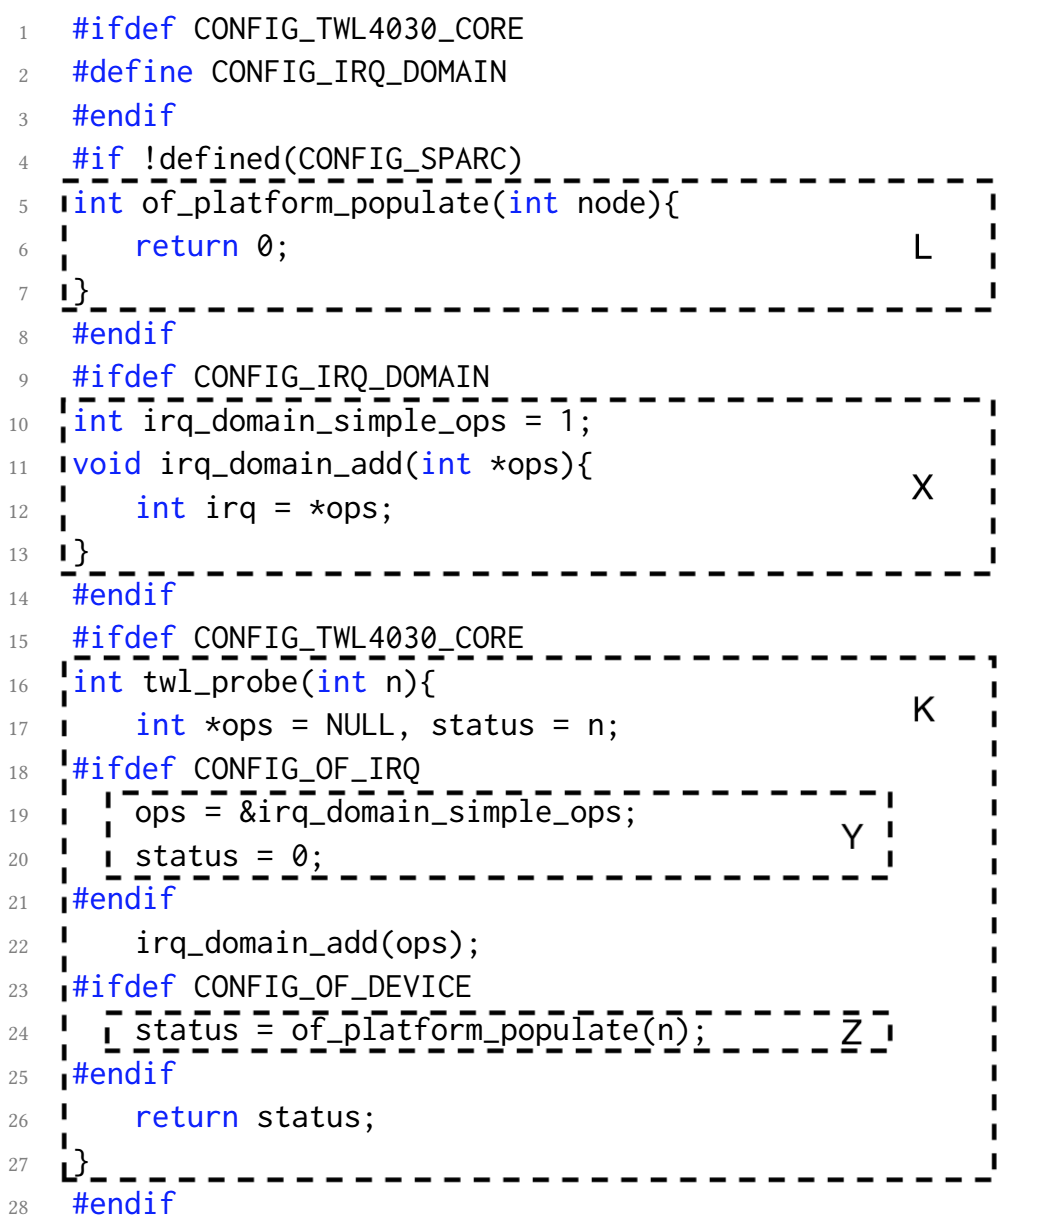
\includegraphics[width=0.5\textwidth]{example_bk.png}
\caption{A simplified buggy version of Linux kernel}
\label{example1}
\end{figure}


\begin{Definition}{({\bf Configuration Option}).}
A configuration option ({\em option} for short) is an element that is used
to configure the source code of a configurable system, such that the
option's value determines the presence or absence of one or more
segments of~code.
\end{Definition}

In a configurable system, the presence or absence of code segments is
dependent on the values of multiple options. In Figure~\ref{example1},
the lines 19 and 20 are presented only when both
\texttt{CONFIG\_TWL4030\_CORE} and \texttt{CONFIG\_OF\_IRQ} are
\texttt{T}. Thus, at line 19, \texttt{irq\_domain\_simple\_ops} is
potentially used to assign as a value to the variable \texttt{ops}
when both above options are \texttt{T}.

%\texttt{CONFIG\_OF\_IRQ} is \texttt{true}.

\begin{Definition}{({\bf Selection Functions}).}
In a configurable system, we define selection functions as the
functions from $O\times V$ to $2^P$, where $O$ is the set of
configuration options, $V=\{\texttt{T, F}\}$, and $P$ is the set of program
entities used in the code of the configurable system. We define four selection functions:

\begin{itemize}

\item $\alpha: O \times V \to 2^P$, $\alpha(o, v) = D$, where $o \in O, v \in \{\texttt{T, F}\}$, and $D$ is the set of entities potentially {\bf declared} if $o = v$.

\item $\beta: O \times V \to 2^P$, $\beta(o, v) = D$, where $o \in O, v \in \{\texttt{T, F}\}$, and $D$ is the set of entities potentially {\bf assigned} if $o = v$.

\item $\gamma: O \times V \to 2^P$, $\gamma(o, v) = D$, where $o \in O, v \in \{\texttt{T, F}\}$, and $D$ is the set of entities potentially {\bf used} if $o = v$.

\item $\delta: O \times V \to 2^P$, $\delta(o, v) = D$, where $o \in O, v \in \{\texttt{T, F}\}$, and $D$ is the set of entities potentially {\bf destructed} if $o = v$.
\end{itemize}

\end{Definition}

For example, in Figure~\ref{example1}:

\begin{itemize}

\item $\alpha($\texttt{CONFIG\_SPARC, F}$)$=$\{$\texttt{GLOBAL.of\_platform\_populate, of\_platform\_populate.node}$\}$

\item $\beta($\texttt{CONFIG\_OF\_IRQ, T}$)$=$\{$\texttt{twl\_probe.ops}$\}$

\item $\gamma($\texttt{CONFIG\_OF\_IRQ, T} $)$=$\{$\texttt{GLOBAL.irq\_domain\_simple\_ops}$\}$

\end{itemize}

\begin{Definition}{({\bf Configuration}).}
Given a configurable system, a configuration is a specific
selection of configuration options, which defines a \textbf{variant}
of the system.
\end{Definition}

Configuration options are used to control the features that are
represented by certain segments of code. For example, in
Figure~\ref{example1}, the feature represented by the segment of code
\texttt{X} (feature \texttt{X}) is enabled if the value of
the configuration option \texttt{CONFIG\_IRQ\_DOMAIN} is \texttt{true},
whereas feature \texttt{Y} is enabled if both \texttt{CONFIG\_OF\_IRQ} and \texttt{CONFIG\_\-TWL4030\_CORE} are \texttt{true}.


The interactions between two features $f_1 \sim OP \times \rho_1$, and
$f_2 \sim OP \times \rho_2$ with $\rho_1 \cap \rho_2 \neq \emptyset$,
can be categorized into nine following kinds of interactions (the
\textit{use-use} case is eliminated):

\begin{itemize}

\item $\exists e \in \rho_1 \cap \rho_2$, $e$ is declared in both $f_1$ and $f_2$ (\textit{declare-declare})

\item $\exists e \in \rho_1 \cap \rho_2$, $e$ is declared in $f_1$ and then assigned in $f_2$ (\textit{declare-assign})

\item $\exists e \in \rho_1 \cap \rho_2$, $e$ is declared in $f_1$ and used in $f_2$ (\textit{declare-use})

\item $\exists e \in \rho_1 \cap \rho_2$, $e$ is declared in $f_1$, and destructed in $f_2$ (\textit{declare-destruct})

\item $\exists e \in \rho_1 \cap \rho_2$, $e$ is assigned in both $f_1$ and $f_2$ (\textit{assign-assign})

\item $\exists e \in \rho_1 \cap \rho_2$, $e$ is assigned in $f_1$ and used in $f_2$ (\textit{assign-use})

\item $\exists e \in \rho_1 \cap \rho_2$, $e$ is assign in $f_1$ and destructed in $f_2$ (\textit{assign-destruct})

\item $\exists e \in \rho_1 \cap \rho_2$, $e$ is used in $f_1$ and destructed in $f_2$ (\textit{use-destruct})

\item $\exists e \in \rho_1 \cap \rho_2$, the entity is destructed in both $f_1$ and $f_2$ (\textit{destruct-destruct})


\end{itemize}


\noindent {\bf Feature Interaction Detection.} In a configurable
system, features (except \textit{the features} in the core of the
system) are controlled by certain configuration options. Thus, if
there exists an interaction among features, the interaction will
be:

\begin{itemize}[leftmargin=4mm]

\item \textit{declare-declare}, there exist two options $o_1, o_2$ and their values $v_1, v_2$, such that $\alpha(o_1, v_1) \cap \alpha(o_2, v_2) \neq \emptyset$

\item \textit{declare-assign}, there exist two options $o_1, o_2$ and their values $v_1, v_2$, such that $\alpha(o_1, v_1) \cap \beta(o_2, v_2) \neq \emptyset$

\item \textit{declare-use}, there exist two options $o_1, o_2$ and their values $v_1, v_2$, such that $\alpha(o_1, v_1) \cap \gamma(o_2, v_2) \neq \emptyset$,

\item \textit{declare-destruct}, there exist two options $o_1, o_2$ and their values $v_1, v_2$, such that $\alpha(o_1, v_1) \cap \delta(o_2, v_2) \neq \emptyset$

\item \textit{assign-assign}, there exist two options $o_1, o_2$ and their values $v_1, v_2$, such that $\beta(o_1, v_1) \cap \beta(o_2, v_2) \neq \emptyset$

\item \textit{assign-use}, there exist two options $o_1, o_2$ and their values $v_1, v_2$, such that $\beta(o_1, v_1) \cap \gamma(o_2, v_2) \neq \emptyset$

\item \textit{assign-destruct}, there exist two options $o_1, o_2$ and their values $v_1, v_2$, such that $\beta(o_1, v_1) \cap \delta(o_2, v_2) \neq \emptyset$

\item \textit{use-destruct}, there exist two options $o_1, o_2$ and their values $v_1, v_2$, such that $\gamma(o_1, v_1) \cap \delta(o_2, v_2) \neq \emptyset$

\item \textit{destruct-destruct}, there exist two options $o_1, o_2$ and their values $v_1, v_2$, such that $\delta(o_1, v_1) \cap \delta(o_2, v_2) \neq \emptyset$

\end{itemize}
\begin{table*}[!h]
\centering
\caption{Different kinds of feature-interaction defects}
\label{bugtypes}
\begin{tabular}{|l|l|l|l|l|}
\hline
&Kind of interaction & Condition & Suspicious selection & Potential violation \\ \hline

1&\textit{declare-declare}&$\alpha(o_1, v_1) \cap \alpha(o_2, v_2) \neq \emptyset$ &$o_1=v_1, o_2=v_2$&Declaration duplication\\ \hline
%2&\textit{declare-assign}&$\alpha(o_1, v_1) \cap \beta(o_2, v_2) \neq \emptyset$&$o_1=v'_1, o_2=v_2$&Assignment without declaration\\ \hline
2&\textit{declare-use}&$\alpha(o_1, v_1) \cap \gamma(o_2, v_2) \neq \emptyset$&$o_1=v'_1, o_2=v_2$&Use without declaration\\ \hline
3&\textit{declare-use}&$\alpha(o_1, v_1) \cap \gamma(o_2, v_2) \neq \emptyset$&$o_1=v_1, o_2=v'_2$&Unused variables/functions\\ \hline
4&\textit{declare-destruct}&$\alpha(o_1, v_1) \cap \delta(o_2, v_2) \neq \emptyset$ &$o_1=v'_1, o_2=v_2$&Destruction without declaration\\ \hline
5&\textit{declare-assign}&$\beta(o_1, v_1) \cap \beta(o_2, v_2) \neq \emptyset$&$o_1=v_1, o_2=v_2$&Assignment without declaration\\ \hline
6&\textit{assign-use}&$\beta(o_1, v_1) \cap \gamma(o_2, v_2) \neq \emptyset$&$o_1=v'_1, o_2=v_2$&Use without assignment\\ \hline
7&\textit{assign-destruct}&$\beta(o_1, v_1) \cap \delta(o_2, v_2) \neq \emptyset$&$o_1=v'_1, o_2=v_2$&Destruction without definition\\ \hline
8&\textit{assign-destruct}&$\beta(o_1, v_1) \cap \delta(o_2, v_2) \neq \emptyset$&$o_1=v_1, o_2=v'_2$&Memory leak\\ \hline
9&\textit{destruct-destruct}&$\delta(o_1, v_1) \cap \delta(o_2, v_2) \neq \emptyset$&$o_1=v_1, o_2=v_2$&Destruction duplication\\ \hline
10&\textit{destruct-use}&$\delta(o_1, v_1) \cap \gamma(o_2, v_2) \neq \emptyset$&$o_1=v_1, o_2=v_2$& Use after destruction\\ \hline
\end{tabular}
\end{table*}


\subsection{Configuration-dependent fault localization}

\textbf{SON: INTRO THE PROBLEM}

\textbf{Overview}
Based on these observations, we propose a novel approach for
configuration-dependent fault localization. The input includes 
the buggy configurable code, the~test result of each
configuration, and the trace of the executed~statements that are
recorded for each test in each configuration, e.g., the trace of the
executed statements in $c_7$ is shown in Fig.~\ref{execution_trace}.

\begin{figure}[h]
\centering
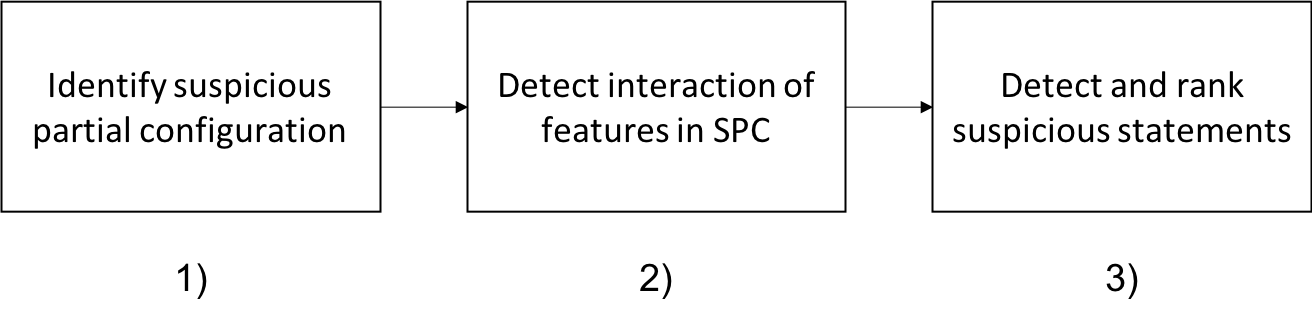
\includegraphics[width=0.7\textwidth]{flowchart}
\label{workflow}
\caption{Approach overview}
\end{figure}
%
In general, to localize a configuration-dependent bug, our algorithm
works in three steps as shown in Fig.~\ref{workflow}.

%
In preprocessor-based program families \cite{kastner2012virtual}, a 
feature selection is controlled by one or more \textit{configuration 
options} (macro symbols). In the example, the feature \texttt{LOCKDEP} 
is controlled by the configuration option \texttt{CONFIG\_LOCKDEP}.
%
In a configurable system, the selections of features are used to specify
particular configurations (variants) of the system.
%
%Configuration
\begin{Definition}{({\bf Configuration}).}
In a configurable system consisting of the set of features $F$, a 
configuration $c$ is a particular set of the selections of all 
features in $F$. We denote $\mathbb{C}$ as the set of all possible 
configurations of the system.
\end{Definition}

In practice, a {\em configuration-dependent} bug can be revealed
during testing, in which there are configurations failing at least
one test, while others pass all their tests.
%
For example, the bug in Fig.~\ref{example_bug} is revealed only in
$c_2$ and $c_7$ in which the features \texttt{LOCKDEP},
\texttt{PPC\_256K\_PAGES}, \texttt{!SLOB}, and \texttt{SLAB} are all
enabled and \texttt{PPC\_16K\_PAGES} is disabled.
%
In highly configurable systems, most of reported bugs  are 
configuration-dependent faults that are only exposed under a set of 
certain configurations \cite{Abal:2018} \cite{Garvin:2011}. 

%

\begin{Definition}{({\bf Configuration-dependent Fault}).}
In a configurable system, a fault of the system is considered as a
configuration-dependent bug if only if there are two non-overlapping
partitions of configurations $CP$ and $CF$, where $CP, CF \subsetneq
\mathbb{C}$, $CF \cup CP = \mathbb{C}$, and $CF \cap CP = \emptyset$,
such that all configurations in $CP$ execute as expected, while all
configurations in $CF$ reveal the bug.
\end{Definition}

\begin{Definition}{({\bf Configuration-dependent Fault Localization}).}
Given buggy configurable code, the test result of each configuration,
and the trace of the executed statements that are recorded for each
test in each configuration, configuration-dependent fault localization
is to output the ranked list of statement(s) that are likely to cause
the fault(s).
\end{Definition}


\input{pc_detection}


\subsubsection{Suspicious Statement Detection}
\label{statement_detection_section}

For a configuration-dependent bug visible by a $SPC$, not only the 
statements that implement the interactions of the features in the 
$SPC$ are likely to be buggy, the executed statements in the failed 
configurations that have dependency impact on them could be suspicious 
as well ({\bf O3} and {\bf O4}).
%considered to be suspicious.
%

Given a $SPC$ of a particular bug, let $ES$ be the set of the statements
that implement the interactions between the enabled features ($f_E$s)
in $SPC$; $DS$ be the set of statements that implement the
interactions of $f_E$s with the disabled features ($f_D$s) in $SPC$.
%
In case that there is no $f_D$ ($DS=\emptyset$), if a statement $smt$
has impact on any statement in $ES$, it is considered as
suspicious. However, in the case that $DS \neq \emptyset$, $smt$ is
considered to be faulty only if $smt$ also has dependency impact on at
least one statement in $DS$. Indeed, because if $smt$ has no
dependency impact on any interaction between $f_E$s and $f_D$s, the
impact of $smt$ is not hidden by any $f_D$ when the features in $f_D$s
are enabled ({\bf O3}).

For the running example, the statements that implement the
interactions of \texttt{SLAB}, \texttt{PPC\_256K\_PAGES},
\texttt{LOCKDEP}, and \texttt{\!SLOB} whose enabling make the bug
visible ($ES$) are the statements at lines 4, 11--12, 16, 22, and
24. These statements are also executed in $c_7$, a failed
configuration, and obviously have impact on the interaction between
features in $ES$.
%
Additionally, another statement that has impact on the interaction is
line 1, and it is also suspicious. However, only the statements at
line 1, 11--12, and 22 have impact on the interactions between
\texttt{PPC\_16K\_PAGES} and the features in $ES$. As a result, for
the bug shown in Fig.~\ref{example_bug}, they are the only suspicious
statements.

\textbf{Suspicious statements ranking.} To rank these suspicious
statements, we analyze the execution information in the testing phase
to assign a suspiciousness score to each of these statements. This
could be realized using spectrum-based
techniques~\cite{wong2009survey}. We use a spectrum-based
tool to access the suspiciousness for only the set of detected
suspicious statements, rather than using them for all executed
statements. Take Tarantula~\cite{tarantula} as an example, the
suspiciousness score of a suspicious statement $stm$:
$$
Suspiciousness(stm) = \frac{N_{CF}/N_F}{N_{CF}/N_F+N_{CS}/N_S}
$$
where:
\begin{itemize}
\item $N_F$ total number of failed test cases
\item $N_S$ total number of successful test cases
\item $N_{CF}$ number of failed test cases that cover $stm$
\item $N_{CS}$ number of successful test cases that cover $stm$
\end{itemize}


%\input{empirical}

%\input{graphsection}

%\input{tool}




%\input{formal}
\section{Education Plan - Curriculum Development Activities}
\label{edu-section}

%From an educational point of view, the central goals of the PI's
%educational plan are: 1) to increase the enrollment and success of
%traditionally under-represented students in engineering, especially in
%Security Engineering and Software Engineering, 2) to integrate
%advanced Secure Software Engineering (SSE) practices into
%undergraduate/graduate courses, 3) and to develop a strong
%undergraduate/graduate SSE program.

%Taking advantage of the newly launched BS degree program in Software
%Engineering at Iowa State University, we would like to directly engage
%and improve the Secure Software Engineering practices of local
%companies. ISU's Computer Engineering Department has an excellent
%foundation on Security research via the Information Assurance
%Center~\cite{iac}. This project will be served as a connection that
%bridges the gap between Information Assurance education and Software
%Engineering education at ISU. The project will strengthen both
%programs.

\noindent {\bf Undergraduate Software Engineering Education.} PI
Nguyen is one of the key SE faculty members in the BS, MS, and Ph.D.
degree programs in Software Engineering (SE) at University of Texas at
Dallas. He has also a track record in contributing to Undergraduate
Education Program when he was at Iowa State University. He has
successfully introduced several courses including Software
Architecture and Design (CprE339) and Software Project Management
(CprE329). Taking advantage of this project, we will introduce a new
course in NLP+SE (natural language processing + software
engineering). The key teaching philosophy in this course is the
combination of theory and practice in which students will be
introduced different principles and theories in the application of NLP
in SE artifacts. The tentative modules include 1) basic principles,
processes, and paradigms in NLP, 2) programming languages versus
natural languages, 3) API usages and reuse, 4) Statisical models used
in SE applications, 5) machine translation and code migration, 6)
language models for source code, 7) applications of machine
translation in SE, 8) word embeddings and SE applications, 9) deep
learning and SE applications, etc.

\noindent {\bf Graduate Software Engineering Education} The PI works
with other UTD faculty to develop a series of six to seven SE graduate
courses that will be offered at least every semester. This year, the
PI introduced a new graduate level course on ``Software Mining and
Analysis''. The PI will introduce a new graduate course on the topic
of NLP+SE. Tools developed by this research will be used in class
projects. The course will focus on several SE advanced methods that
aim to help advance software engineering with NLP techniques. The
tentative topics include 1) bug report processing, 2) source code
analysis with NLP, 3) cross-language analysis between texts and code,
4) code and text retrieval in SE applications, 5) NLP techniques and
type inference, 6) NLP and de-ofuscation, 7) bug-fixing and
machine learning, 8) NL+SE for big data, etc.


%%%Some of these modules have been introduced to students at ISU as part
%%%of the BS Software Engineering degree program and several programs at
%%%the Information Assurance center\cite{iac}.

%The results from the security domain analysis will be used in all five
%components. The proposed RSD method, SSADL specification, and design
%supporting tools will be used in the teaching components in
%(B). 

%Efforts will be made to involve minority graduate students recruited
%by ISU through GEM and NSF AGEP programs. Currently, PI serves as a
%mentor for the Leadership through Engineering Academic Diversity
%(LEAD) programs which aims to enrich the educational experience of
%minority engineering students on the ISU campus. Participants in ISU's
%Women in Science and Engineering will be given the opportunity to
%participate in the proposed research. Annually, there are Security
%Summer Camps for high-school students and faculty, organized by ISU's
%Information Assurance Center. These events allow us to involve
%minority students and faculty into the proposed research.

\input{dissemination.tex}

\section{Evaluation Plan}
\label{eval-section}

Our {\em goals} of the evaluation plan include the studies to answer the questions:

1) {\bf Intrinsic evaluation.} How accurate are our mining and API
usage code synthesis approaches, and how well are they in comparison
with the state-of-the-art approaches?

2) {\bf Extrinsic evaluation.} How well do our proposed tools and methods help developers in
improving the learning and usages of APIs in software libraries?

3) How effectively do the proposed tools and methods help developers
in real development processes?

%1) the
%evaluation the understanding of the characteristics and nature of API
%misuses related to security vulnerabilities and their corresponding
%causes, 2) the evaluation of identification methods for potential
%API-misuses related vulnerabilities, and 3) the evaluation of the
%quality of the suggested locations/components and recommendations for
%a new vulnerability in a new system. 

%For the goal~1, the correctness in the understanding of
%characteristics and the representation of API-related vulnerabilities
%will be evaluated in the performance evaluation of techniques and
%tools built for detecting potential vulnerabilities and
%recommendations. To achieve the goals 2 and 3, we plan to perform {\em
%  empirical evaluation} tasks. Let us next provide the details for
%those evaluation tasks.

\subsection{Instrinsic Evaluation of the proposed Code Mining and API Usage Synthesis}

First, we will perform automatic evaluation on the accuracy of the
constructed text-API usage code snippet pairs. We plan to
automatically build a corpus as gold-standard data. We will mine the
StackOverflow data collected in Rigby and
Robillard~\cite{rigby-icse13}. In the dataset, we currently use
236,919 entries, each of which has two parts: 1) the textual
descriptions of the usage/purpose of some programming task, and 2) the
corresponding bag of API elements that are extracted from the posts
(including from its descriptions and code snippets). The posts and
code elements were extracted via the ACE tool. We will expand the
dataset for further evaluation. We compare the inferred bags of
elements against the bags of API elements for those posts in the
StackOverflow dataset. We will then measure the precision, recall, and
F-measure of the pairs that are automatically extracted using our
techniques.  Recall is defined as the ratio between the number of
elements that appear in both the actual and inferred bags of elements
and the number of actual API elements. Precision is the ratio between
the number of API elements that appear in both the actual and inferred
bags of elements and the number of inferred elements.

For API usage synthesis approaches, we will use the code snippets in
the above dataset. However, we will compare the generated API usages
against those code snippets. We will use the metrics on {\em syntactic
correctness} (how well do the code compile and run), and {\em semantic
correctness} (how well do the code match the desired API usages).

\subsection{Evaluation on usefulness of the approaches in helping
developers in learning API usages}

We will perform controlled experiments to evaluate our methods and
tools with developers in the loop using the actual system. We will
gather developers and provide them various programming tasks, and
compare the efficiency of their work with our methods/tools to the
baseline approaches, e.g., with the Web-based code search or other
code synthesis approaches.

We will measure the efficiency of the work using different methods
based on the following evaluation metrics. First, we measure
efficiency. This could be measured by the time for developers to
perform the tasks or the number tasks completed by developers in a
period of time. Second, we measure coding effort: how much effort that
developers must do to complete the API usages given the API code from
the methods. Third, we will measure semantic correctness, either by
the number of passing test cases or by human judgements. Finally, we
will perform surveys on the quality of the synthesized API usage code
to get the feedback for future improvement in the next step.


\subsection{Evaluation on  proposed tools and methods in helping developers
in real-world development}

We will perform a set of user studies on the usefulness of our
proposed IDE tools and Web-based tools in the wild by releasing our
tools in the actual real-world development. We will analyze all the
aspects as in the previous studies, as well as the frequency of usage
of code suggestions, and the total uptake of the tools.  We will track
the changes that developers make to the generated code and record
their feedback to improve our tools.

We will work with our collaborators in Microsoft, IBM, and ABB research
to perform user studies on the groups of developers in certain tasks
to evaluate the usefulness of our proposed tools.

\section{Project Schedule and Expected Milestones}
\label{plan-section}

The PI has broken the proposed activities into subtasks with
tentative milestones:


1. Ongoing Empirical Studies to mine a large-scale parrallel corpus of
text and code.
   
2. Work on Context-aware Inferrence of Relevant APIs to a Textual Query.

3. Work on Deriving Fully-Qualified Types for APIs in Incomplete Code
in StackOverflow.


4. API Usage Code Synthesis: Models, Representations, and
Methodologies

\hspace{0.1in}   3.1. Graph-based Representations

\hspace{0.1in}   3.2. Graph Synthesis Models and API usage code synthesis.


4. Integrating Code Synthesis into Developer Assistance Tools

\hspace{0.1in}   4.1. Developer assistance tools in IDE.

\hspace{0.1in}   4.2. Web-based developer assistance tools.


5. The integration of the associated tools and their
deployment/training for evaluation, and

6. Evaluation, education, dissemination, and publications.

%====================================================================

\noindent {\bf Year 1}: We focus our ongoing effort to expand our
ongoing on empirical studies in task 1. We will focus also on tasks 2
and 3, and expect to finish task 2 by the end of year 1.

\noindent {\bf Year 2}: We will finish task 2 in the first 3 months of
this year. Tasks 3,4, and 5 will be in our focus in year~2.

\noindent {\bf Year 3}: The prototype integration will
begin. Publications will begin as soon as we have new results.
Education dissemination will start. We will focus on evaluation, and
continue publications and dissemination.

%The foundation consists of both the open architectural CM (task 1) and
%the formulation of flow control and configurable policies (task 2). By
%the end of year 1, we expect to finish task 2. Task 1 could last
%around 14-15 months.

%Year 2: We will start the implementation of that CM architecture
%and supporting tools. In this year, more study will be done for
%conflict problem in GSD

%We also begin the implementation of associated tools for CCM in task
%4. Model merge/synchronization framework (task 5) will be
%continued. Education components will be implemented and publications
%will begin to pick up.

%Year 3: We will change our focus to CCM model and the implementation
%of its associated tools (tasks 4 and 5). Some testing and integration
%will begin. We will continue the publication and dissemination.

%Year 4: We expect to produce most of important results in tasks
%1,2,3,4, and 5. The evaluation will begin.

%Year 5: We will focus on evaluation, testing, integration, and
%continue the publications and dissemination.

%\input{priorsupport}
\section{PI's Prior Relevant NSF Supports and Qualifications for this Project}
\label{prior-section}

CCF-1723215, \$260,709, 07/01/16-30/06/18, ``Collaborative
Research: Exploiting the Naturalness of Software''. 
%
\noindent {\bf Intellectural Merit.} The work has three thrusts of
research: (1) Investigating the integration of semantic information
including data types, semantic roles, etc., into a language model, (2)
Developing an accurate code-completion tool using statistical semantic
language model, and (3) Developing a statistical machine translation
model for language migration.
%
\noindent {\bf Broader Impact.} We will transform practical software
engineering tools, using statistical NL techniques, introducing new
generations of (a) code suggestion, completion, and correction tools,
(b) assistive tools for programmers, (c)
summarization, (d) retrieval, and (e) porting tools.  Our work will
help reduce the dominant maintenance component of the software
industry.

%making software development more accessible, enjoyable and productive;
%and therefore will broadly enhance the value that software
%professionals deliver to business and society.

%Dr. Nguyen is currently the PI of the NSF-funded project, ``
%Collaborative Research: Exploiting the Naturalness of Software'', that
%will end August 2018. The work has three thrusts of research.  (1)
%Investigating the integration of semantic information including data
%types, semantic roles, etc., into a language model, (2) Developing an
%accurate code-completion tool using statistical semantic language
%model, and (3) Developing a statistical machine translation model for
%language migration. So far, the majority of the tasks have been
%%completed except empirical evaluation in a real-word setting is
%needed. 

The project has been resulting several publications at top-tier SE
conferences including ICSE
papers~\cite{icse05,icse07,icse09,icse10,icse11}, FSE
papers~\cite{fse06,fse09,fse11}, ASE
papers~\cite{ase06,ase08,ase08-2,ase09,ase10,ase11-phpsync,ase11-bugscout,ase11-idiff},
OOPSLA papers~\cite{oopsla04,oopsla06,oopsla10}, and TSE
papers~\cite{tse08,tse11}.

%Several papers on our results were published through ICSE
%2010~\cite{icse10}, ASE 2010~\cite{ase10}, OOPSLA
%2010~\cite{oopsla10}, ICSM 2010~\cite{icsm10}, ICSE
%2011~\cite{icse11,nier11-1,nier11-2}, FSE 2011~\cite{fse11}, ASE
%2011~\cite{ase11-phpsync,ase11-bugscout,ase11-idiff}, and an IEEE TSE
%journal article~\cite{tse11}.

%Our next phase will be involved more with the tasks (2) and (3).

%Dr. Nguyen is currently an PI on a NSF-funded project: \#CCF-1018600,
%``Find and Fix Similar Software Bugs'', 08/15/2010 through
%07/31/2013. In this project, an empirical study will be conducted to
%collect, analyze, and understand the nature and characteristics of
%recurring and similar bugs within one and across multiple
%systems. This project is expected to advance software engineering
%knowledge on the theoretical foundation, concepts, practical
%techniques, and automated tools to (1) capture the characteristics and
%measure the similarity of code units involved in prior known fixed
%bugs, (2) identify the locations of potential buggy units and derive
%the guidelines to fix them by matching them to the relevant peer code
%units of the known bugs, and (3) support the similar bug detection and
%fixing process. Teaching modules and validation efforts in this
%project will involve students and professionals, promoting teaching
%and training software quality assurance.

%Dr. Nguyen is an expert in software building, software configuration
%management (SCM), and software refactoring. His research work on SCM
%has been published at various prestigious software engineering
%journals and conferences including clone-aware configuration
%management and operation-based version control (TSE'11~\cite{tse11},
%FASE'10~\cite{fase10}, ASE'09~\cite{ase09}), software
%refactoring-aware SCM and software merging (TSE'08 \cite{tse08},
%ICSE'07~\cite{icse07}, FSE'06~\cite{fse06}, OOPSLA'06
%demo~\cite{oopsla06}), object-oriented configuration management
%(ICSE'07~\cite{icse07}, WWW'06~\cite{www06}, ICSE'05~\cite{icse05},
%ICSM'05~\cite{icsm05}).

His other software maintenance works include clone-related bug
detection (TSE'11 \cite{tse11}), bug localization
(ASE'11~\cite{ase11-phpsync}), bug localization from bug reports
(ASE'11~\cite{ase11-bugscout}), recurring bug detection
(ICSE'10~\cite{icse10}), API misuse detection
(OOPSLA'10~\cite{oopsla10}, FSE'09~\cite{fse09}), recurring
vulnerabilities detection (ASE'10~\cite{ase10}), etc.  He was a
Program Co-Chair of the 32nd ACM/IEEE International Conference on
Automated Software Engineering (ASE 2017).

Since 2009, he has been awarded {\bf 4 ACM SIGSOFT Distinguished Paper
Awards, one Best Paper Award, and one best ICSE Formal Research
Demonstration Award} at the top-tier, international software
engineering conferences including ICSE, FSE, and ASE. He is the
Co-Chair of the Formal Research Demo Track at the 40th International
Conference on Software Engineering (ICSE 2018) and the International
Symposium on the Foundations of Software Engineering (FSE 2018). He
has served on Program Committees and Program Boards of top-tier
software engineering conferences: ICSE, FSE, ASE, OOPSLA,
ECOOP.


%Since 2005, his work has been resulting several publications at
%top-tier SE conferences including 5 ICSE
%papers~\cite{icse05,icse07,icse09,icse10,icse11}, 3 FSE
%papers~\cite{fse06,fse09,fse11}, 8 ASE
%papers~\cite{ase06,ase08,ase08-2,ase09,ase10,ase11-phpsync,ase11-bugscout,ase11-idiff},
%2 WWW papers~\cite{www04,www06}, 3 OOPSLA
%papers~\cite{oopsla04,oopsla06,oopsla10}, and 2 FASE
%papers~\cite{fase09,fase10}, 2 TSE papers~\cite{tse08,tse11}.


\newpage
\setcounter{page}{1}
\pagenumbering{roman}

\bibliographystyle{IEEEtran}

\bibliography{tien,ccf18}

%icse18,t2api17,ccf18,refs,securesync,tc10,tien,ccf09,ase10,ccf12,anomalies,completion,groums,usagemining,pattern,urls,other}

\end{document}
